% -*- TeX:de -*-
\NeedsTeXFormat{LaTeX2e}
\documentclass[12pt,a4paper]{article}
\usepackage[german]{babel} % german text
\usepackage[DIV12]{typearea} % size of printable area
\usepackage[T1]{fontenc} % font encoding
%\usepackage[latin1]{inputenc} % most likely on Windows
\usepackage[utf8]{inputenc} % probably on Linux
\usepackage{multicol}

% PLOTTING
\usepackage{pgfplots} 
\usepackage{pgfplotstable}
\usepackage{url}
\usepackage{graphicx} % to include images
\usepackage{tikz}
\usepackage{subfigure} % for creating subfigures
\usepackage{amsmath} % a bunch of symbols
\usepackage{amssymb} % even more symbols
\usepackage{booktabs} % pretty tables
\usepackage{makecell} % multi row table heading

% a floating environment for circuits
\usepackage{float}
\usepackage{caption}

%\newfloat{circuit}{tbph}{circuits}
%\floatname{circuit}{Schaltplan}

% a floating environment for diagrams
%\newfloat{diagram}{tbph}{diagrams}
%\floatname{diagram}{Diagramm}

\selectlanguage{german} % use german

\begin{document}

%%%%%%% DECKBLATT %%%%%%%
\thispagestyle{empty}
			\begin{center}
			\Large{Fakultät für Physik}\\
			\end{center}
\begin{verbatim}


\end{verbatim}
							%Eintrag des Wintersemesters
			\begin{center}
			\textbf{\LARGE SS 14}
			\end{center}
\begin{verbatim}


\end{verbatim}
			\begin{center}
			\textbf{\LARGE{Physikalisches Praktikum\\ für das Bachelorstudium}}
			\end{center}
\begin{verbatim}




\end{verbatim}

			\begin{center}
			\textbf{\LARGE{PROTOKOLL}}
			\end{center}
			
\begin{verbatim}

\end{verbatim}

			\begin{flushleft}
			\textbf{\Large{Experiment (Nr., Titel):}}\\
							%Experiment Nr. und Titel statt den Punkten eintragen
			\LARGE{PS05 Polarisation}	
			\end{flushleft}

\begin{verbatim}

\end{verbatim}	
							%Eintragen des Abgabedatums, oder des Erstelldatums des Protokolls
			\begin{flushleft}
			\textbf{\Large{Datum:}} \Large{13.3.2014}
			\end{flushleft}
			
\begin{verbatim}
\end{verbatim}
							%Namen der Protokollschreiber
		\begin{flushleft}
			\textbf{\Large{Namen:}} \Large{Patrick Braun, Johannes Kurz}
			\end{flushleft}

\begin{verbatim}


\end{verbatim}
							%Kurstag und Gruppennummer, zb. Fr/5
			\begin{flushleft}
			\textbf{\Large{Kurstag/Gruppe:}} \Large{DO/4}
			\end{flushleft}

\begin{verbatim}

\end{verbatim}
							%Name des Betreuers, das Praktikum betreute.
			\begin{flushleft}
			\LARGE{\textbf{Betreuer:}}	\Large{Erhard Schafler}	
			\end{flushleft}

%%%%%%% DECKBLATT ENDE %%%%%%%
\pagebreak
\setlength{\columnsep}{20pt}
\begin{multicols}{2}

%%%%%%%%%%%%%%%%%%%%%%%%%%%%%%%%%%%%%%%%%%%%%%%%

%\begin{figure}[H]
%	\centering
%	\includegraphics[scale=0.35]{./data/beugung.png}
%	\caption{Beugungsmuster Einzelspalt (echtes Foto; schwarz durch weiß ersetzt)}
%	\label{fig:beugungsmuster}
%\end{figure}


%\begin{figure}[H]
%	\centering
%	\pgfplotstabletypeset[
%			columns={abstand, n},
%			col sep=&,
%			columns/abstand/.style={precision=2, zerofill, column name=\makecell{$Abstand$\\$(\pm 0.05)[mm]$} }, 
%			columns/n/.style={column name=\makecell{$n$\\$(Ordnung)$}, precision=0},
%			every head row/.style={before row=\hline,after row=\hline\hline},
%			every last row/.style={after row=\hline},
%			every first column/.style={column type/.add={|}{} },
%			every last column/.style={column type/.add={}{|} }
%			]{
%			abstand & n
%			12.9 & 1
%			24.45 & 2
%			37.40 & 3
%			49.35& 4
%			62.45 & 5
%			74.45 & 6
%			87.45 & 7
%			100.25 & 8
%			
%			}
%	\caption{Messwerte Einzelspalt}
%	\label{tab:werte_einzelspalt}
%\end{figure}



%%%%%%%%%%%%%%%%%%%%%%%%%%%%%%%%%%%%%%%%%%%%%%%%
%%%%%%%%%%%%%%%%%%%%%%%%%%%%%%%%%%%%%%%%%%%%%%%%
\section{Grundlagen, Theorie und Versuchsaufbau}

\subsection{Brewster Winkel}
Durch die Eigenschaft von Licht, aus vertikalen und horizontalen Komponenten zu bestehen, wird bei einer Einstrahlung von Licht auf einen Körper (z.B. von Luft auf Glas) nur ein Teil reflektiert. Genau jener Anteil der senkrecht auf die Einfallsebene steht.\\
Ist Licht nur einfach polarisiert und zwar senkrecht zur Einfallsebene, wird immer weniger Licht reflektiert, bis nur noch Hintergrundrauschen fest zu stellen ist.\\ 
Der Winkel des einbestrahlten Lichtes, bei dem nichts reflektiert wird, heißt Brewster Winkel.\\
Ein einfacher geometrischer Zusammenhang beschreibt wie folgt den Winkel:

$$tan(\alpha_B) = \frac{n_2}{n_1}$$


\begin{figure}[H]
	\centering
	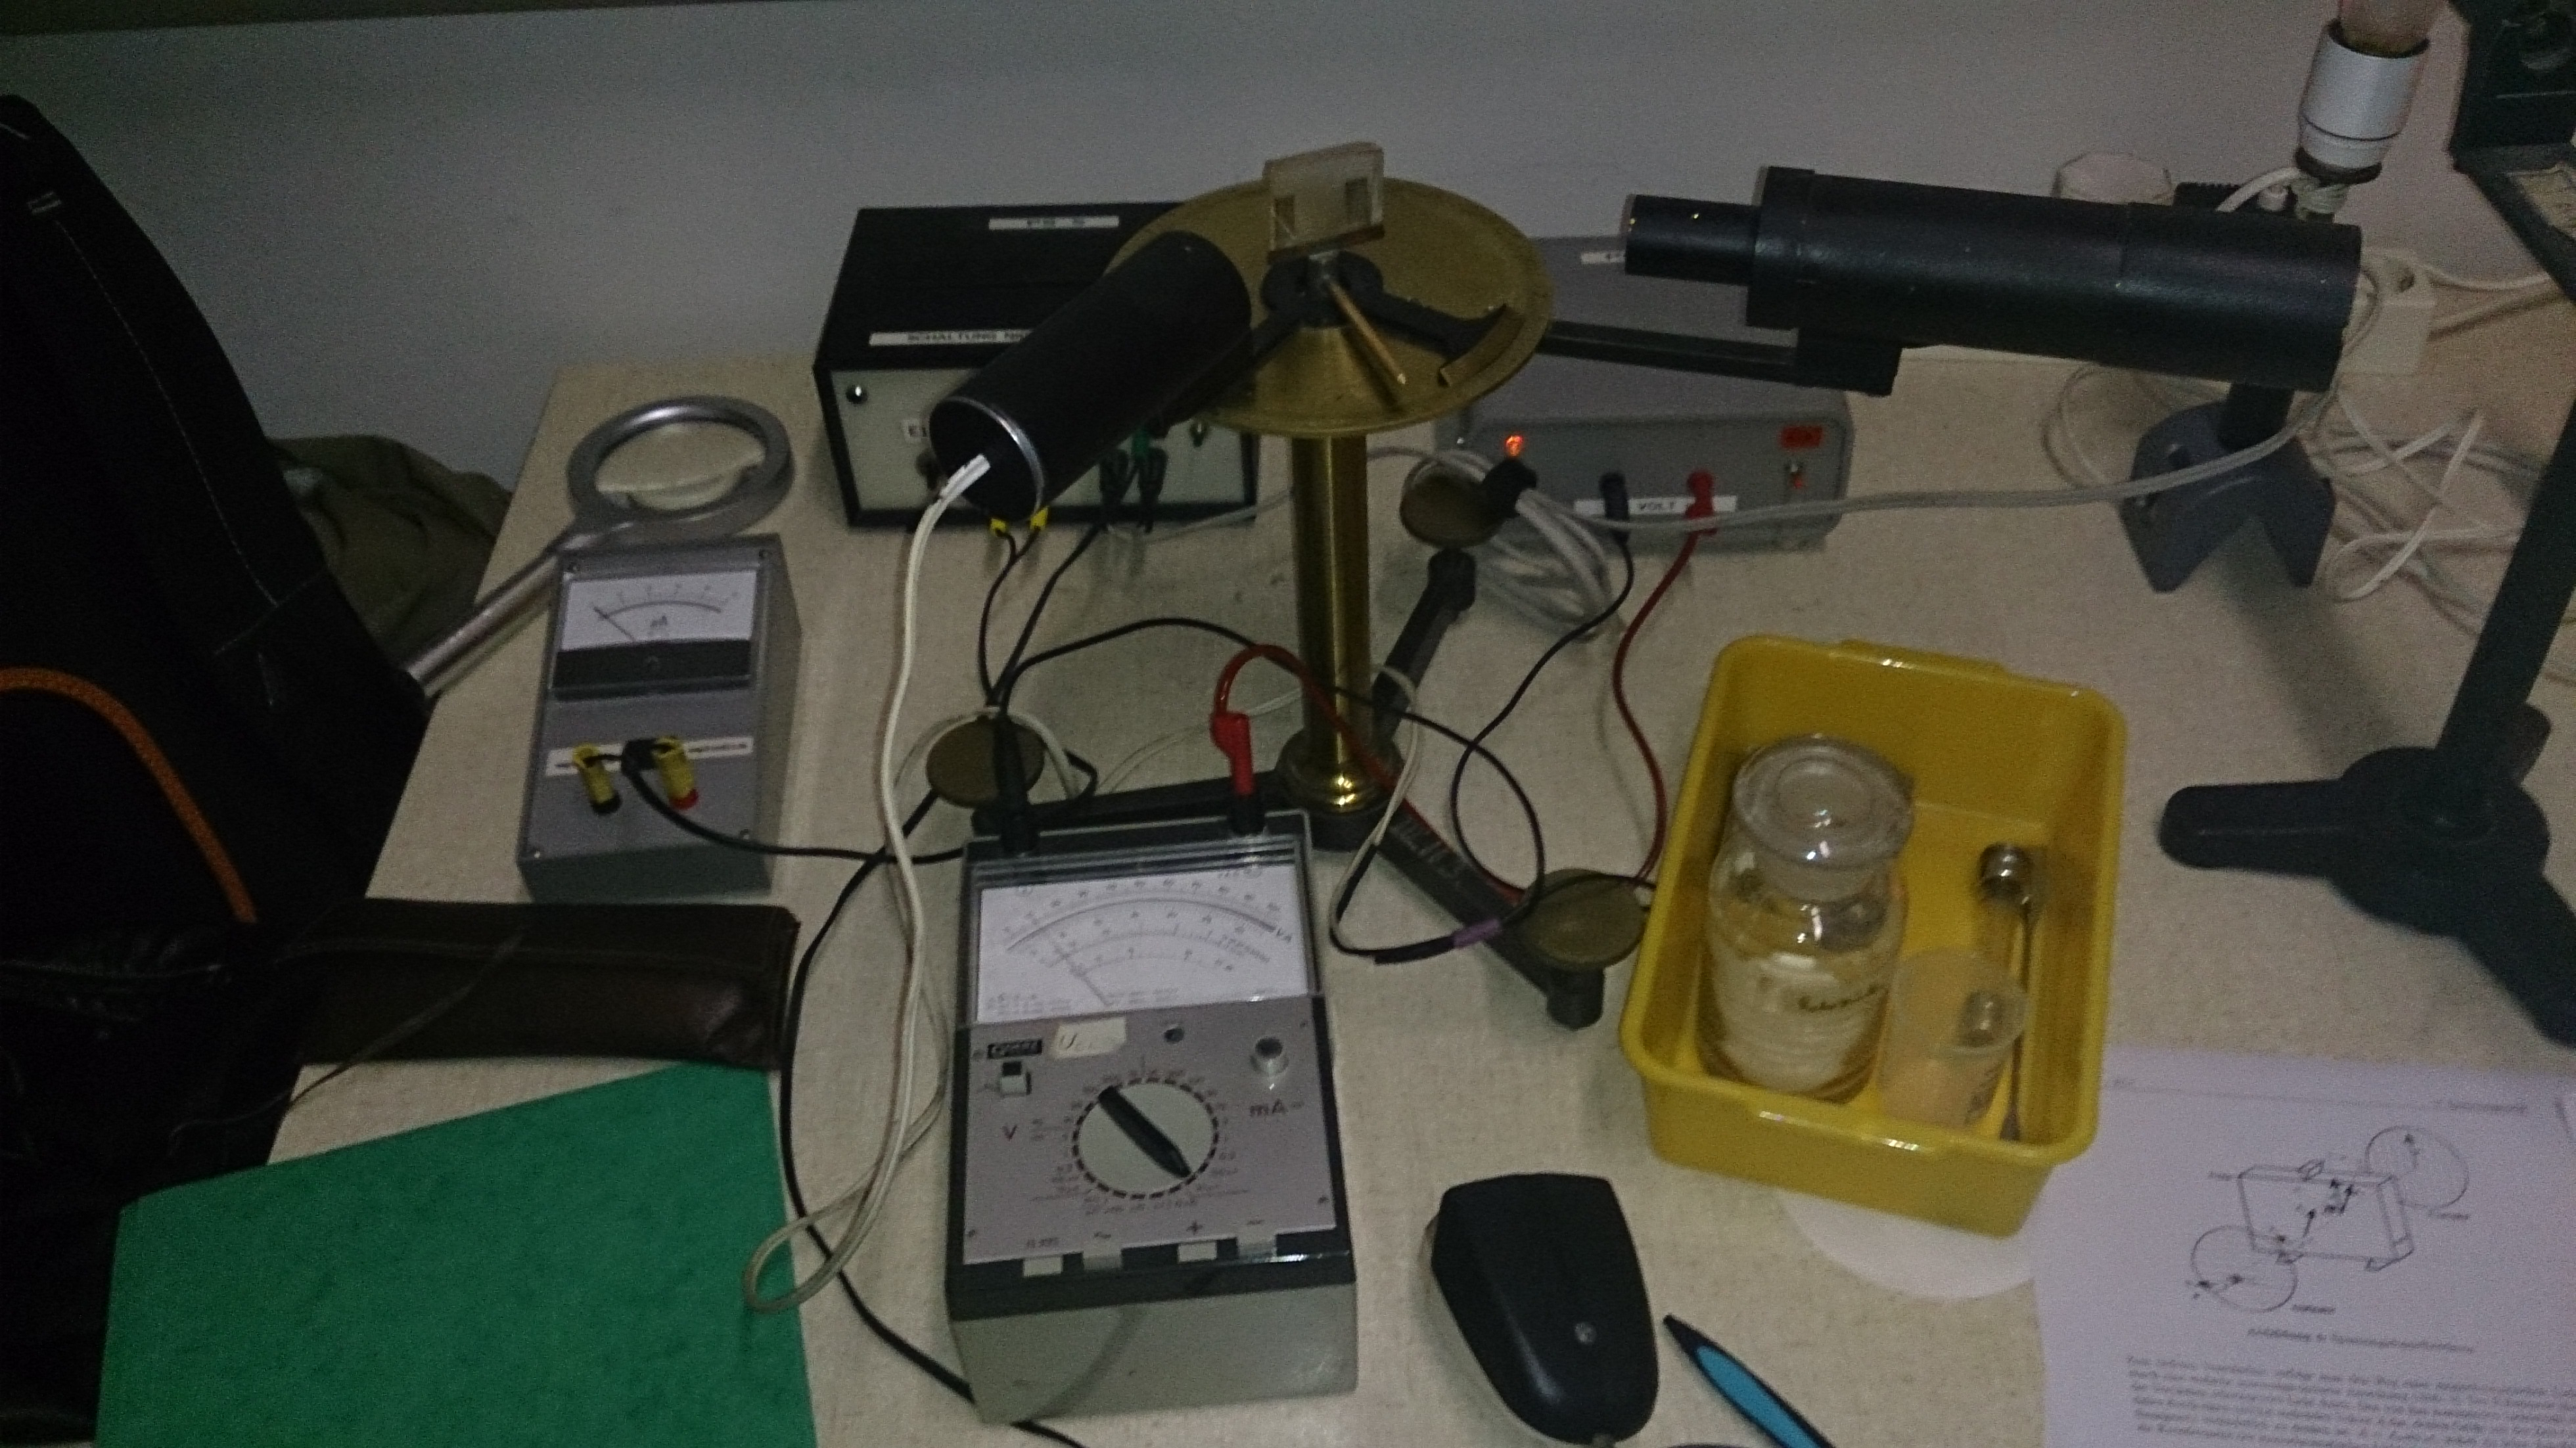
\includegraphics[scale=0.1]{./data/PS5_1_Aufbau.jpg}
	\caption{Aufbau zur Messung des Brewster Winkel}
	\label{fig:brewster_aufbau}
\end{figure}

\begin{figure}[H]
	\centering
	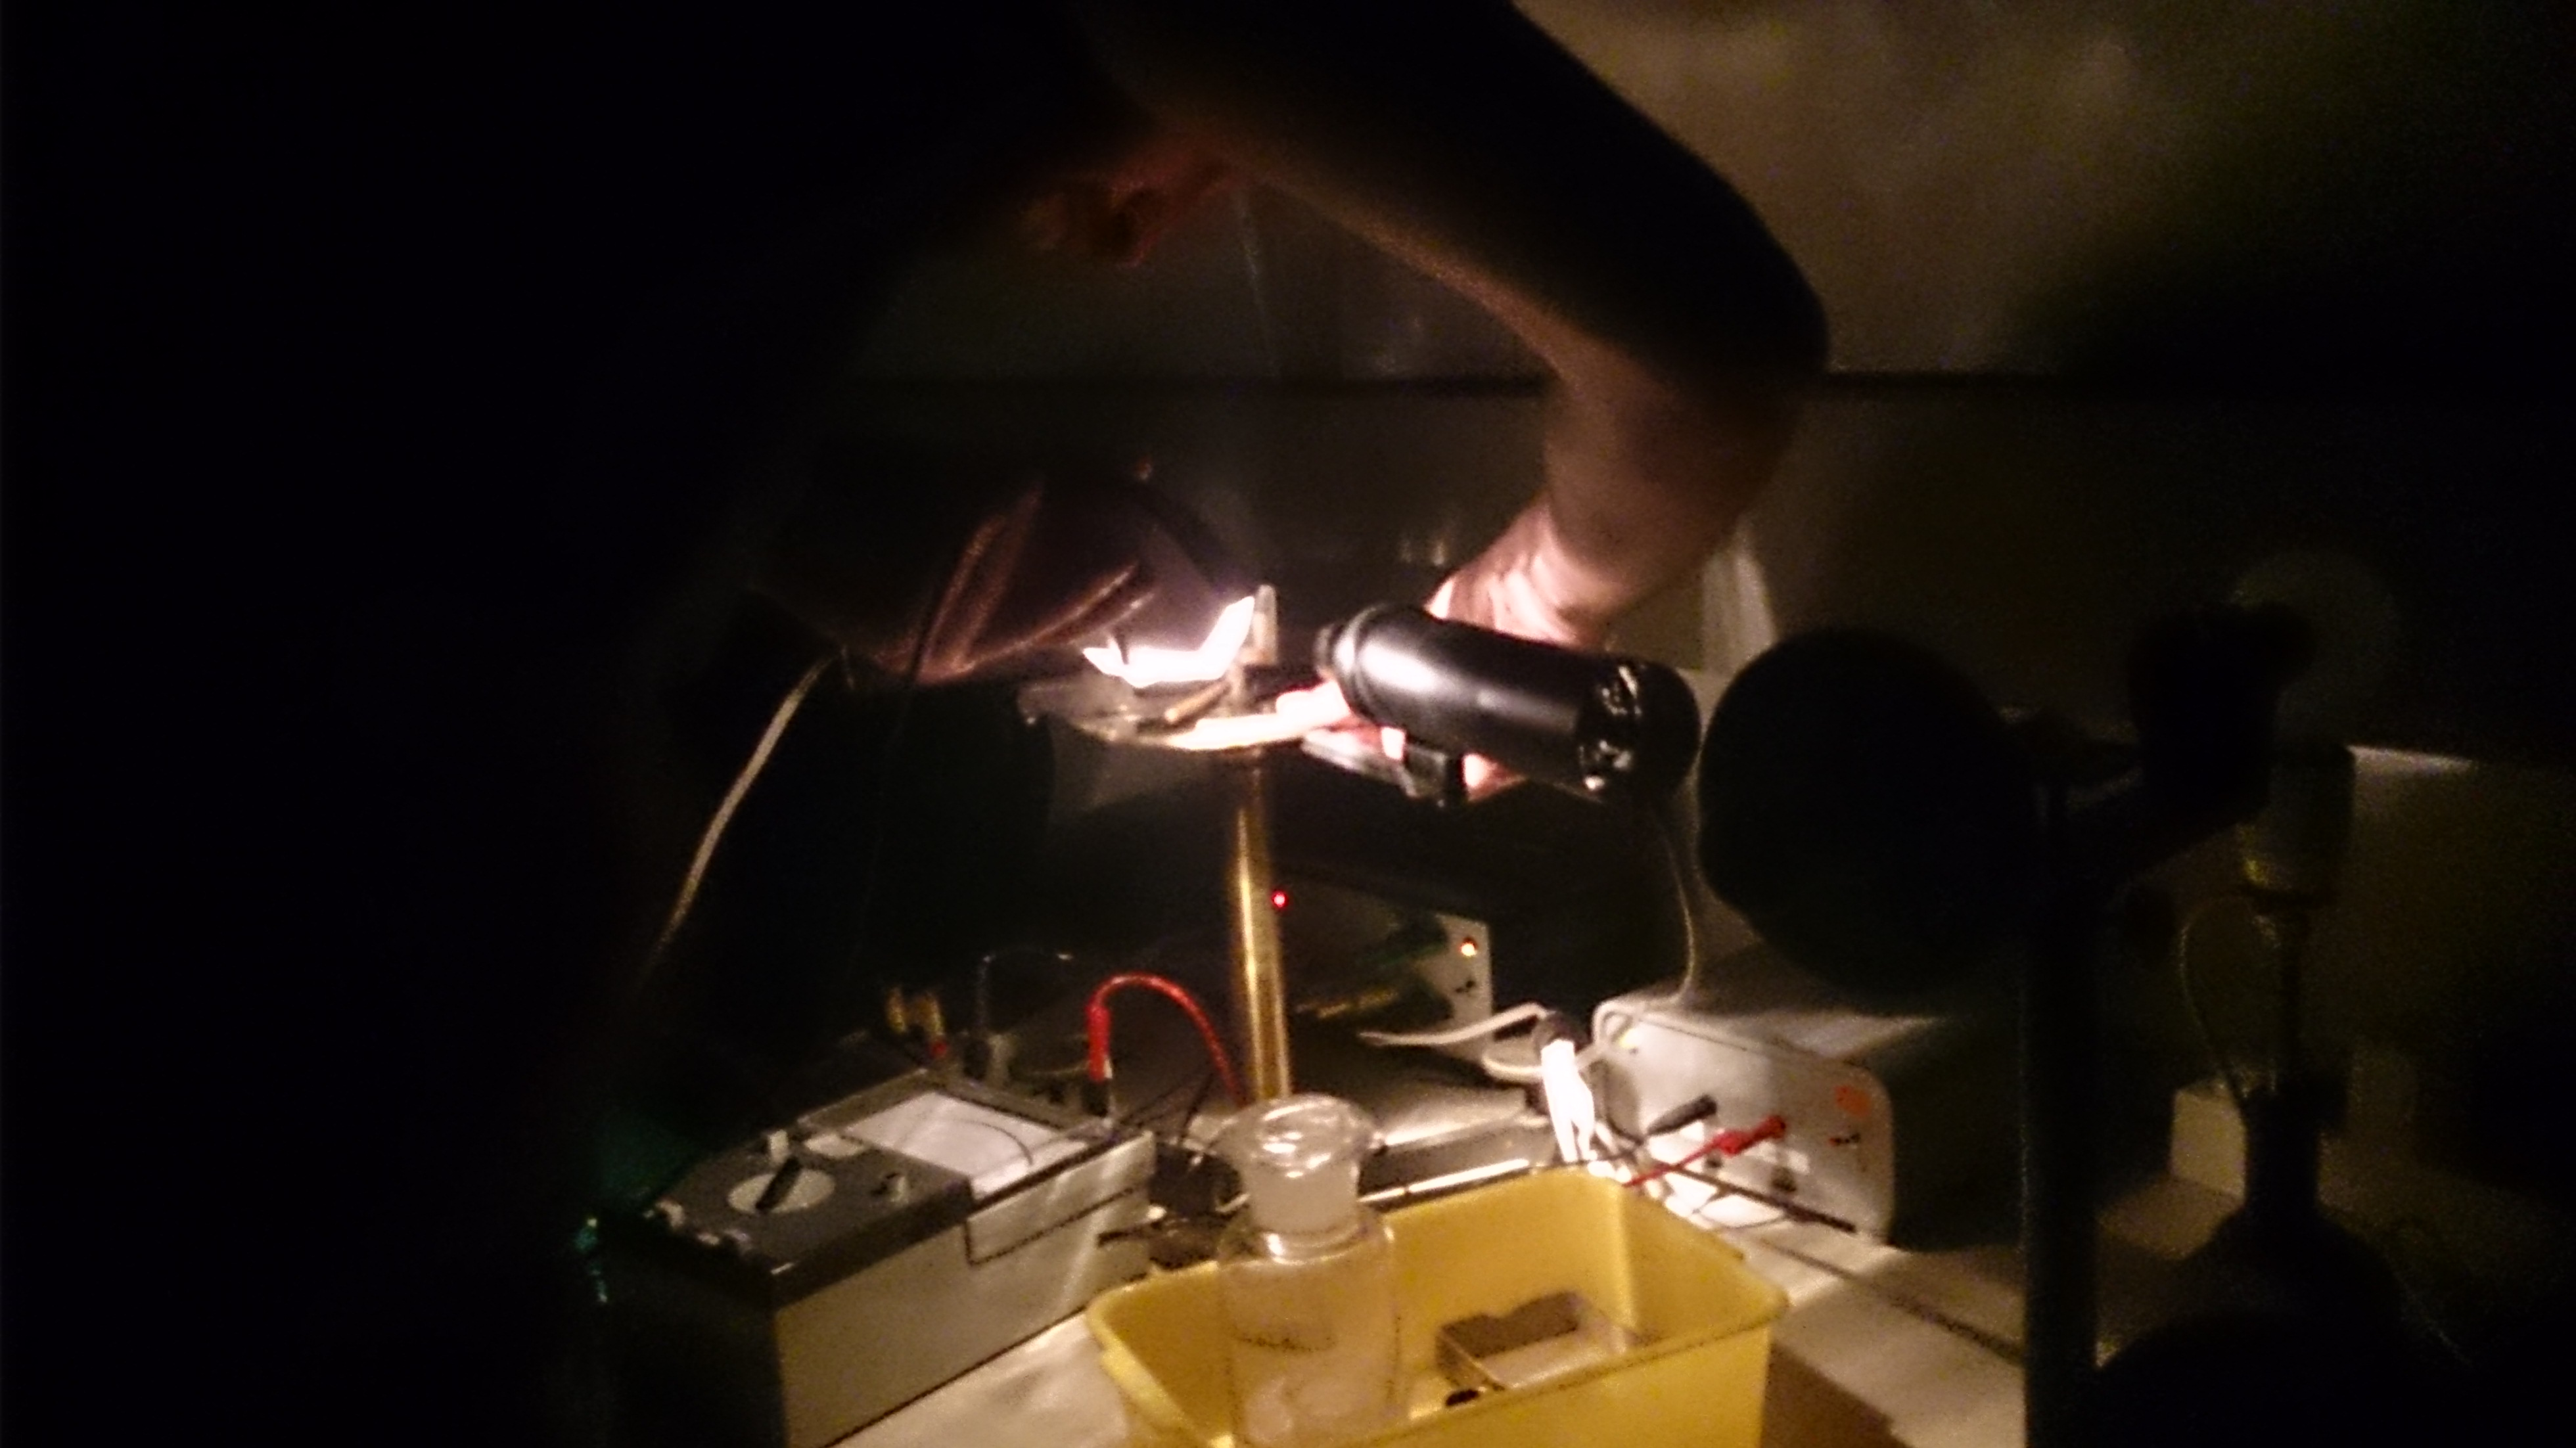
\includegraphics[scale=0.1]{./data/PS5_1_Justierung.jpg}
	\caption{Nachjustierung zur Messung des Brewster Winkel}
	\label{fig:brewster_justierung}
\end{figure}

\subsection{Spannungsoptik}

\begin{figure}[H]
	\centering
	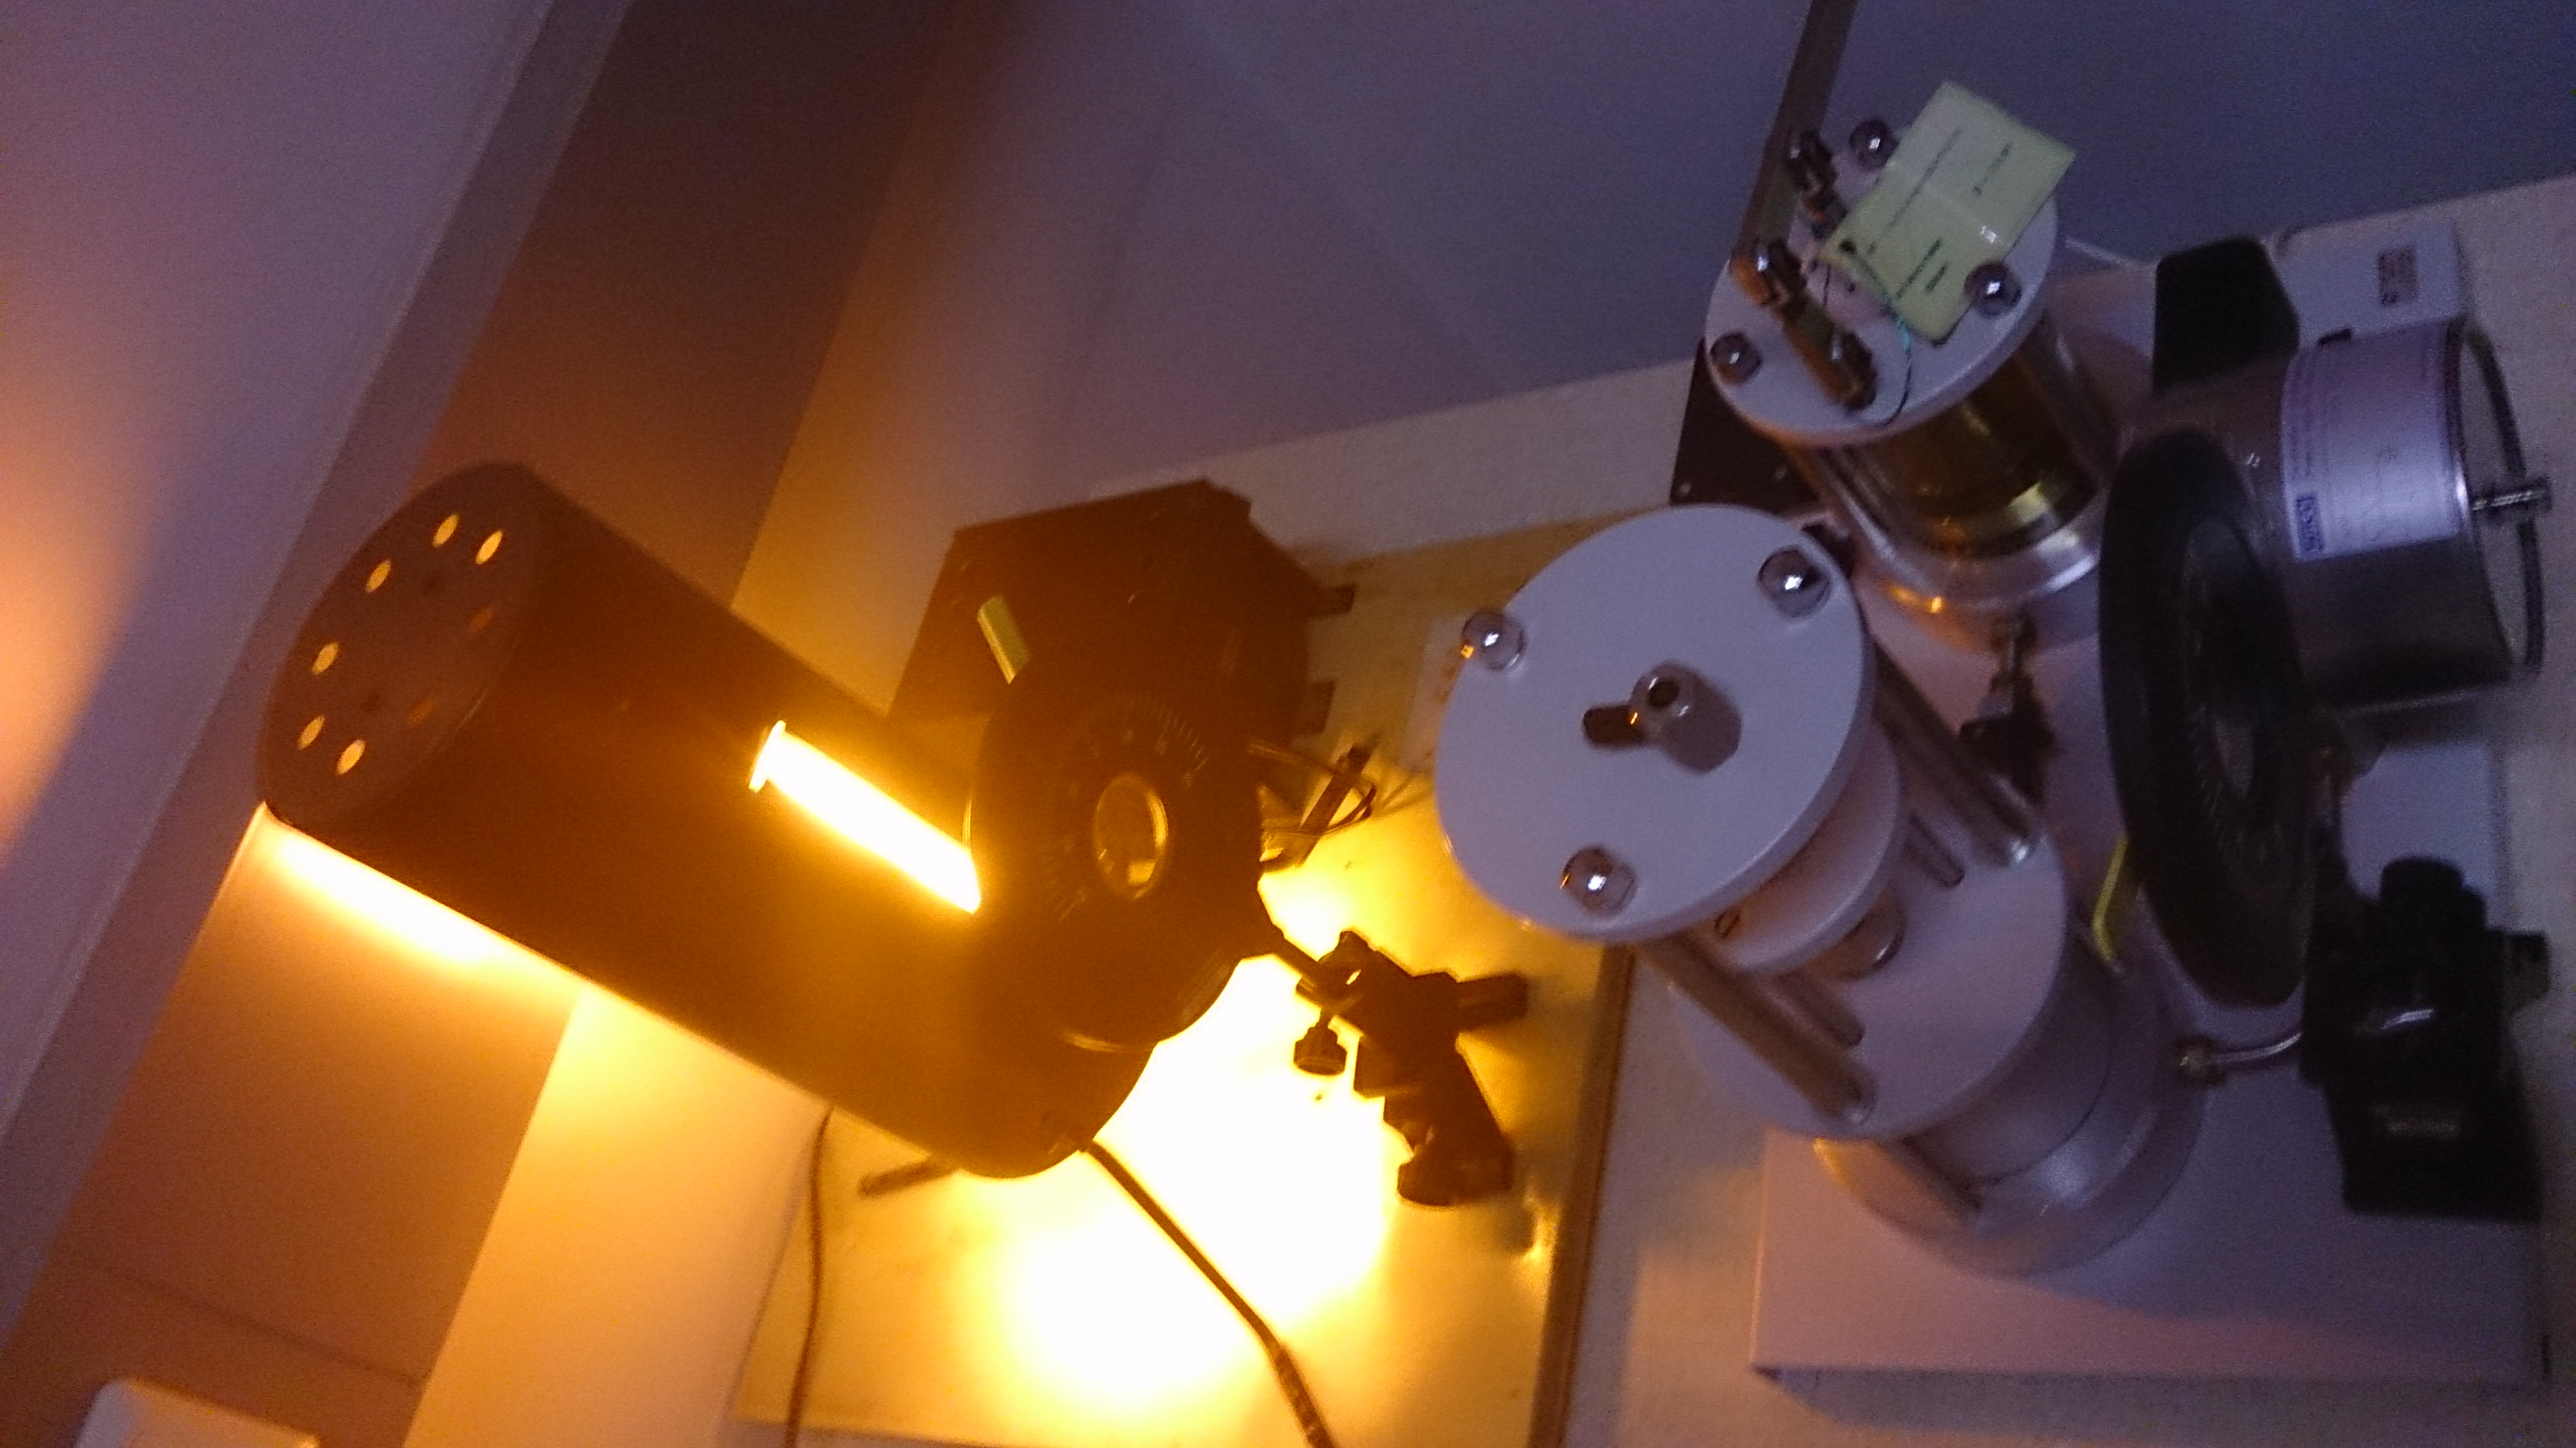
\includegraphics[scale=0.1]{./data/PS5_2_Aufbau.jpg}
	\caption{Aufbau zur optischen Messung einer Doppelbrechung}
	\label{fig:spannung_aufbau}
\end{figure}

\begin{figure}[H]
	\centering
	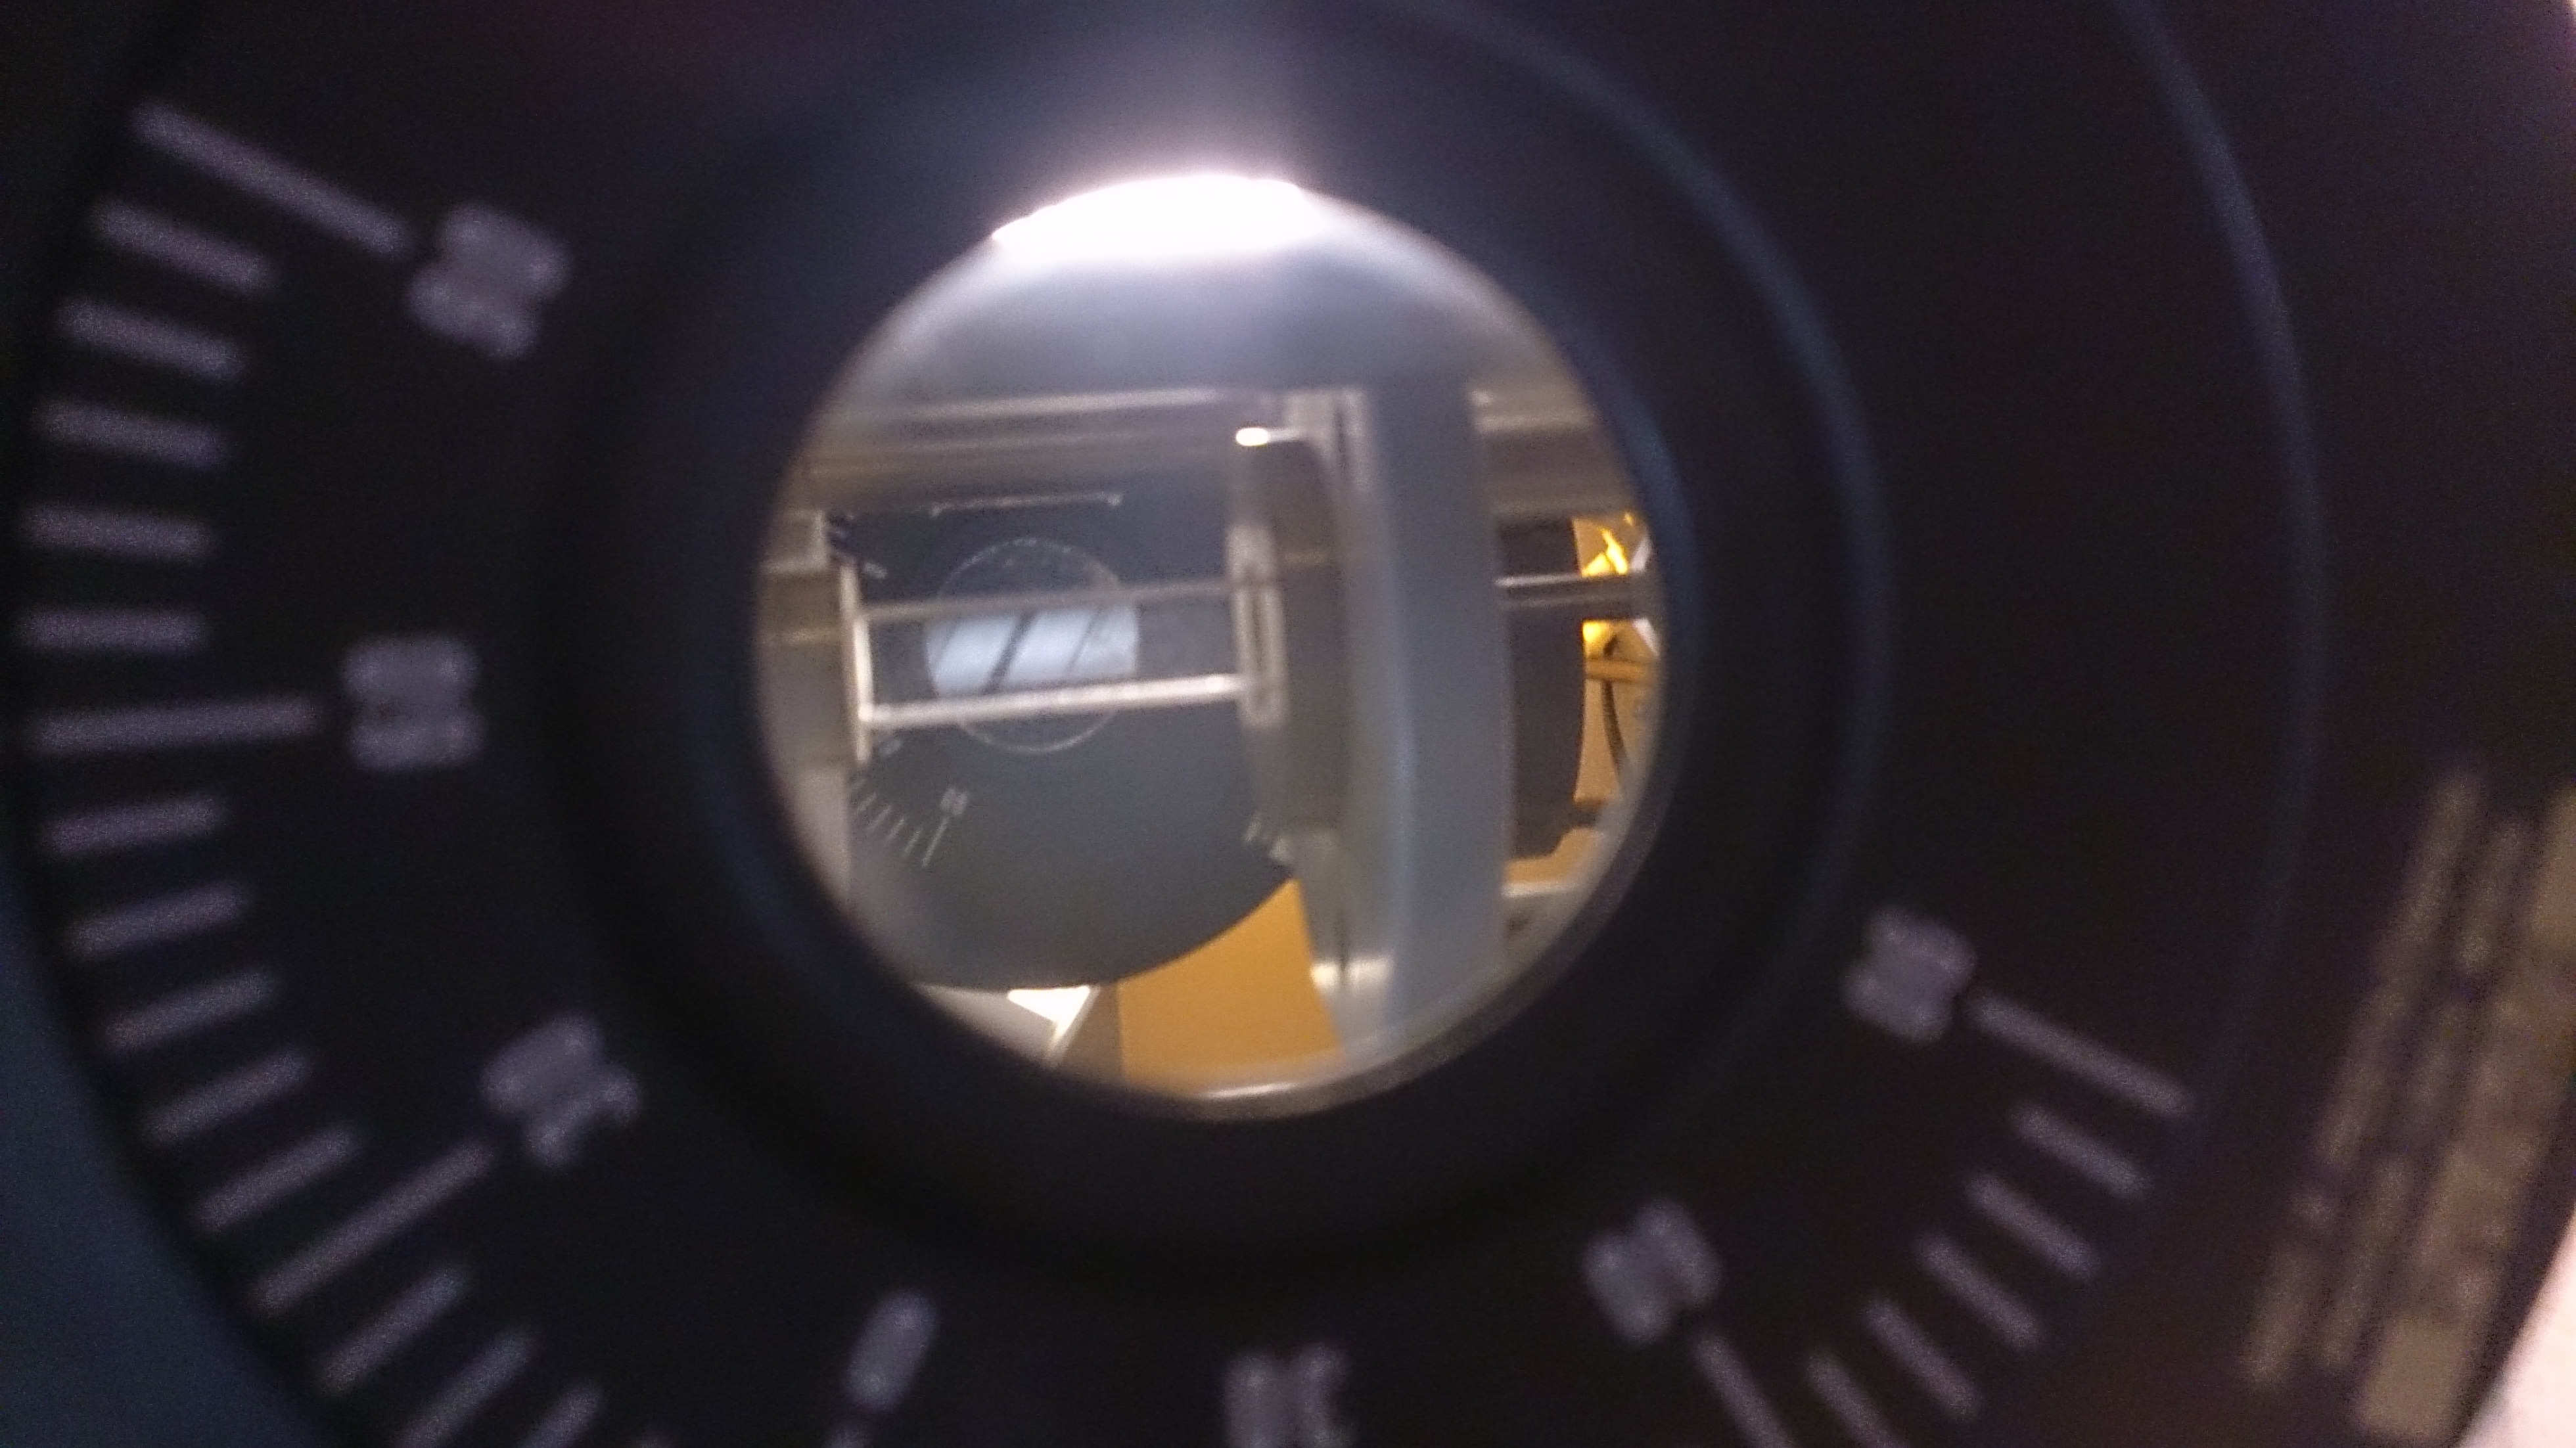
\includegraphics[scale=0.1]{./data/PS5_2_Filterjustierung.jpg}
	\caption{Justierung der Polarisationsfilter mit weißem Licht}
	\label{fig:spannung_justierung}
\end{figure}

\subsection{Drehung der Polarisationsebene}

%TODO Bild aus Anleitung oder so

%%%%%%%%%%%%%%%%%%%%%%%%%%%%%%%%%%%%%%%%%%%%%%%%
%%%%%%%%%%%%%%%%%%%%%%%%%%%%%%%%%%%%%%%%%%%%%%%%
\section{Resultate}

\subsection{Brewster Winkel}



\subsection{Spannungsoptik}




\subsection{Drehung der Polarisationsebene}




%%%%%%%%%%%%%%%%%%%%%%%%%%%%%%%%%%%%%%%%%%%%%%%%
%%%%%%%%%%%%%%%%%%%%%%%%%%%%%%%%%%%%%%%%%%%%%%%%
\section{Diskussion}

\subsection{Brewster Winkel}



\subsection{Spannungsoptik}




\subsection{Drehung der Polarisationsebene}




\section{Quellen}
$[1]$ Anleitung, \url{http://www.univie.ac.at/anfpra/neu1/ps/ps5/PS5.pdf}\\
\end{multicols}

\end{document}